\pdfoutput=1

\documentclass[10pt,letterpaper]{article}

\usepackage[utf8]{inputenc} % allow utf-8 input
\usepackage[T1]{fontenc}    % use 8-bit T1 fonts
\usepackage{lmodern}
\usepackage{hyperref}       % hyperlinks
\usepackage{url}            % simple URL typesetting
\usepackage{booktabs}       % professional-quality tables
\usepackage{amsfonts}       % blackboard math symbols
\usepackage{nicefrac}       % compact symbols for 1/2, etc.
\usepackage{microtype}      % microtypography
\usepackage{xspace}
\usepackage{authblk}

\usepackage{graphicx}
\graphicspath{{pictures/}}
\usepackage{amsmath}
\usepackage{amssymb}
\usepackage{amsthm}
\usepackage{bm}
\usepackage[margin=1in]{geometry}

\usepackage[font=small]{caption}
\usepackage{subcaption}
\usepackage{tikz}
\usepackage{pgfplots}
\usepackage{fp}
\usetikzlibrary{bayesnet}

\theoremstyle{plain}
\newtheorem{thm}{Theorem}[section]
\newtheorem{lem}[thm]{Lemma}
\newtheorem{prop}[thm]{Proposition}
\newtheorem*{cor}{Corollary}

\theoremstyle{definition}
\newtheorem{defn}{Definition}[section]
\newtheorem{conj}{Conjecture}[section]
\newtheorem{exmp}{Example}[section]

\theoremstyle{remark}
\newtheorem*{rem}{Remark}
\newtheorem*{note}{Note}

\DeclareMathOperator*{\argmin}{arg\,min}
\newcommand{\normk}[1] {\left\| #1 \right\|_k}
\newcommand{\norm}[1] {\left\| #1 \right\|}
\newcommand{\abs}[1] {| #1 |}
\newcommand{\normtwo}[1] {\left\| #1 \right\|_2}
\newcommand{\normf}[1] {\left\| #1 \right\|_{\mathcal{F}}}
\newcommand{\frob}[1]{\|#1\|_\mathcal{F}}
\newcommand{\sumz}{\sum_{z=1}^Z}
\newcommand{\sumi}{\sum_{i=1}^m}
\newcommand{\sump}{\sum_{p=1}^L}
\newcommand{\sumiz}[1]{\sum_{#1=1 | z_{#1}=z}^m}
\newcommand{\sumik}[1]{\sum_{#1=1 | k_{#1}=k}^m}
\newcommand{\sumk}{\sum_{k=1}^L}
\newcommand{\mul}[1] {{\mu}_{\mkern-0.66\thinmuskip\mathcal{L}} (#1) }

\newcommand{\wrt}{w.r.t.\@\xspace}

\newcommand\todo[1]{\textcolor{red}{#1}}
\renewcommand\todo[1]{}

\newcommand{\twocol}[2]{
    \begin{tabular}{cc}
        #1 & #2 
    \end{tabular}
}

\newcommand{\landSVM}{L$^3$-SVMs\xspace}

\author[1]{Zantedeschi Valentina \\
\href{mailto:valentina.zantedeschi@univ-st-etienne.fr}{valentina.zantedeschi@univ-st-etienne.fr}}
\author[1]{\\Emonet R\'emi\\
\href{mailto:remi.emonet@univ-st-etienne.fr}{remi.emonet@univ-st-etienne.fr}}
\author[1]{\\Sebban Marc\\
\href{mailto:marc.sebban@univ-st-etienne.fr}{marc.sebban@univ-st-etienne.fr}}

\affil[1]{
Univ Lyon, UJM-Saint-Etienne, CNRS, Institut d Optique Graduate School, Laboratoire Hubert Curien UMR 5516, F-42023, SAINT-ETIENNE, France
}

\title{\landSVM: \\Landmarks-based Linear Local Support Vector Machines}
\date{}

\begin{document}

\maketitle


\begin{abstract}
For their ability to capture non-linearities in the data and to scale to large training sets, local Support Vector Machines (SVMs) have received a special attention during the past decade. 
In this paper, we introduce a new local SVM method, called \landSVM, which clusters the input space, carries out dimensionality reduction by projecting the data on landmarks, and jointly learns a linear combination of local  models. Simple and effective, our algorithm is also theoretically well-founded. Using the framework of Uniform Stability, we show that our SVM formulation comes with generalization guarantees on the true risk. 
The experiments based on the simplest configuration of our model (i.e. landmarks randomly selected, linear projection, linear kernel) show that \landSVM is very competitive \wrt the state of the art and opens the door to new exciting  lines of research.
\end{abstract}
Reinforcement learning has achieved great success in areas such as Game-playing \citep{silver2018general,vinyals2019grandmaster}, robotics \cite{kober2013reinforcement}, large language models \citep{ouyang2022training}, etc.
However, due to safety concerns or physical limitations, in some real-world reinforcement learning problems, we must consider additional constraints that may influence the optimal policy and the learning process \citep{garcia2015comprehensive}.
% For example, a robotic arm must not take actions that may cause harm to itself or the environments.
A standard framework to handle such cases is the constrained Markov Decision Process (CMDP) \citep{altman1999constrained}.
Within the CMDP framework, the agent has to maximize
the expected cumulative reward while
obeying a finite number of constraints, which are usually in the form of expected cumulative cost criteria.

However, we are sometimes concerned with the problem with a continuum of constraints.
For example,
the constraints we meet might be time-evolving or subject to uncertain parameters, which
cannot be formulated as an ordinary CMDP
(see Examples \ref{Example_Time_Evolving} and  \ref{Example_Uncertain}).
In this paper we would study a generalized CMDP  
to address the above problem.  Because the constraints are not only infinite-number but also lie
in a continuous set,
the generalization is not trivial. Fortunately, we find that we can borrow the idea behind semi-infinite programming (SIP) \citep{remez1934determination, hettich1993semi} to deal with the semi-infinite constraints.
Accordingly, we propose \emph{semi-infinitely constrained Markov decision processes} (SICMDPs)
as a novel complement to the ordinary CMDP framework.
%More specifically,  an SICMDP model %, we consider 
%contains a continuum of constraints whereas an ordinary CMDP contains a finite number of constraints. 

%This generalization is natural but not trivial. However, we can brows the idea  
%The idea is quite natural and can be backtracked
%to the practice of extending linear programming to linear semi-infinite programming (LSIP) %\cite{remez1934determination, GobernaLSIO1998}.
%In addition, 
%As a complementary approach to the ordinary CMDP framework, 
%SICMDP can be used to model these problems  which cannot be described by a finite number of constraints
%that are not covered by .
%For example,
%the restrictions we consider can be time-evolving or subject to uncertain parameters
%, thus
%cannot be described by a finite number of constraints but a continuum of constraints 
%(see Examples \ref{Example_Time_Evolving} and  \ref{Example_Uncertain}).

We also present two reinforcement learning algorithms to solve SICMDPs called SI-CRL and SI-CPO, respectively.
SI-CRL is a model-based reinforcement learning algorithm designed for tabular cases, and SI-CPO is a policy optimization algorithm for non-tabular cases.
% and analyze its performance both theoretically and empirically.
The main challenge is that we need to deal with a continuum of constraints, thus reinforcement learning algorithms for ordinary CMDPs do not work anymore.
In SI-CRL, we tackle this difficulty by first transforming the reinforcement learning problem to an equivalent LSIP problem, which can then be solved using methods in the LSIP literature like the dual exchange methods \citep{Hu1990,reemtsen1998numerical}.
In SI-CPO, we resort to the idea of cooperative stochastic approximation developed in \cite{lan2020algorithms, wei2020comirror}.
As far as we know, we are the first to introduce tools from semi-infinitely programming (SIP) into the reinforcement learning community for solving constrained reinforcement learning problems.

% To the best of our knowledge, we are the first to apply tools from semi-infinitely programming (SIP) to solve reinforcement learning problems.
Furthermore, we give theoretical analysis for both SI-CRL and SI-CPO.
We decompose the error of SI-CRL into two parts: the statistical error from approximating the true SICMDP with an offline dataset and the optimization error due to the fact that the solution of the LSIP problem obtained by the dual exchange method is inexact.
On the optimization side, we show that the iteration complexity of SI-CRL is $O\left(\left\{\mathrm{diam}(Y)L\sqrt{|\gS|^2|\gA|m}/\left[(1-\gamma)\epsilon\right]\right\}^m\right)$.
On the statistical side, we show that the sample complexity of SI-CRL is $\widetilde O\left(\frac{|S|^2|A|^2}{\epsilon^2(1-\gamma)^3}\right)$ if the offline dataset is generated by a generative model, and $\widetilde O\left(\frac{|S||A|}{\nu_{\min} \epsilon^2(1-\gamma)^3}\right)$ if the dataset is generated by a probability measure $\nu$ as considered in \cite{chen2019information}.
Here $\widetilde O$ means that all logarithm terms are discarded.
For SI-CPO, things become a little more complicated because other than the statistical error and the optimization error, we also need to consider the function approximation error, which comes from imperfect policy parametrizations.
It is shown if the function approximation error can be controlled to $O(\epsilon)$ order, the iteration complexity of SI-CPO is $\widetilde{O}\left(\frac{1}{\epsilon^2(1-\gamma)^6}\right)$ and the sample complexity of SI-CPO is $\widetilde{O}(\frac{1}{\epsilon^4(1-\gamma)^{10}})$.
Here our iteration complexity bound is equivalent to a typical $\widetilde O(1/\sqrt{T})$ global convergence rate.

We perform a set of numerical experiments to illustrate the SICMDP model and validate our proposed algorithms.
Specifically, we examine two numerical examples, namely the discharge of sewage and ship route planning.
Through the discharge of sewage example, we show the advantage of the SICMDP framework over the CMDP baseline obtained by naive discretization in modeling realistic sequential decision-making problems.
Moreover, we demonstrate the effectiveness of the SI-CRL and SI-CPO algorithms in such tabular environments. 
In the ship route planning example, we illustrate the benefits of the SICMDP framework and the ability of the SI-CPO algorithm to address complex continuous control tasks involving continuous state spaces with modern deep reinforcement learning techniques.

% In summary, our contributions are listed as follows.
% First, we present the SICMDP model, which can be viewed as a generalization of the ordinary CMDP model.
% Second, we propose an algorithm to perform reinforcement learning for SICMDPs, which is called SI-CRL, and we believe that we are the first to apply tools from SIP
% to solve reinforcement learning problems.
% Third, we give a theoretical analysis of SI-CRL and identify both its sample complexity and iteration complexity.
% In addition, we perform numerical experiments to illustrate the SICMDP model and validate the SI-CRL algorithm.
% \{This paragraph can be removed!!! \}





The proposed segmentation-by-detection framework, as depicted in Figure \ref{fig:framework}, consists of a detection module and a segmentation module.
In detection stage, 2D slices (layered box) from the input volume are fed to the RPN. Based on the region proposals obtained from RPN, an attention model (block in orange) is formed. The input volume as well as the attention model are further processed in segmentation stage to get the refined anatomical segmentation. 
\vspace{1em} 

\begin{figure}[t]
\centering
\includegraphics[width=0.95\linewidth]{fig/framework.pdf}
\caption{Schematic representation of the segmentation-by-detection framework. The left part is the detection module while the segmentation module is followed on the right. The blue block denotes the input volume which is 3D ultrasound scan of femoral head. The output segmentation is in red.}
\label{fig:framework}
\end{figure}
% dana could you improve the figure. we can try to think together of better ways 

\noindent\textbf{Detection Module:} 
% dana : here you have to make the clarification that you have ground truth on the boxes (in implementation part)
The detection module follows an RPN architecture, a fully convolutional network which takes image slice as input and outputs object region candidates. 
We use the VGG-16 model as the backbone \cite{simonyan2014very} to learn convolutional features and an $3 \times 3$ spatial window to generate region proposals. At each sliding-window location, 9 anchors are predicted associated with different scales and aspect ratios. The last layer consists of a box-regression (reg) layer and a box-classification (cls) layer in parallel. The reg layer outputs 4 regression offsets, $ t = (t_x,t_y,t_w,t_h)$, denoting a scale-invariant translation as well as log-space height and width shift, where $x,y,w$ and $h$ specify two coordinates of the box center, width and height. The cls layer outputs two scores by softmax, related to probabilities of object and background for each proposal. We assign a positive label (of being object) to candidate which has an Intersection-over-Union (IoU) ratio higher than 0.7 with ground truth box. Note that an image slice may contain multiple object regions or none. 

The loss function of RPN follows the multi-task loss \cite{ren2015faster} which is defined as $L = L_{reg} + L_{cls}$. The regression loss, $L_{reg} = -\log p_{obj}$ is log loss and the classification loss,
\begin{equation} \label{eq:loss}
L_{cls} = \sum_{i \in \{x,y,w,h\}} smooth_{L_1} (t_i - t_i^*)
\end{equation}
is smooth $L_1$ loss where $t_i^*$ denotes the ground truth box for the target object. 
\vspace{1em}

\noindent\textbf{Segmentation Module:}
3D U-Net \cite{cciccek20163d} is utilized in the segmentation module as its outstanding performance in medical image segmentation. The u-shaped architecture consists of two paths: a contracting path, where each layer contains two $3\times3\times3$ convolutions followed by a rectified linear unit (ReLU) and then a max pooling, provides high resolution features. While, the symmetric expanding path for semantically richer features replaces max pooling with a upconvolution $2\times2\times2$ with stride of 2 in each dimension, and then two $3\times3\times3$ convolutions each followed by a ReLU. Skip connections between layers of equal resolution in the contracting path and the expanding path enables context information as well as precise localization.

Different from 3D U-Net, to incorporate the attention model detected by the RPN, our architecture takes as input both the volumetric image data and the candidate RoIs proposed by the RPN, concatenated as 3D volume. 
% dana not sure what you like to say below
% densely annotated
The attention model makes the network to focus on the potential RoIs and can reduce the interference of the surrounding noise.
The anatomical segmentation is then generated from a $1\times1\times1$ convolution which reduces the number of feature maps to the number of labels.  The energy function is computed by a pixel-wise softmax combined with the cross entropy loss.
% dana equation ??

\subsection{System and implementation Details}
The segmentation-by-detection approach adopts a cascade structure with two stages: detection and segmentation. The two networks are trained separately in an end-to-end manner. All the new layers are randomly initialized from zero-mean Gaussian distribution with standard deviations 0.01. Biases are initialized to 0. We use Caffe \cite{jia2014caffe} for the implementation and an NVIDIA Titan X GPU for training.

In the detection stage, we initialize the VGG-16 model by the pre-trained model for ImageNet classification \cite{russakovsky2015imagenet} and further fine-tune the model for our detection task. The input fed to the network are image slices with a fixed size of $184\times96$ and the corresponding ground truth boxes are generated from the annotation in the format of tight bounding boxes surrounding the segmentation contour (as illustrated in Figure \ref{fig:hip} (b), the boundary of white area). To optimize the energy function, stochastic gradient descent (SGD) is used. The global learning rate is set to 0.001, while a momentum of 0.9 and a weight decay of 0.0005 are used. The batch size is set to 256 and each mini-batch only contains the positive anchors for training. The region proposals are obtained from the reg path for each image slice. The attention model is then formed by concatenating all the detected regions, as binary masks, into a volume.

In the segmentation stage, we use the Adam optimizer \cite{kingma2014adam} to learn the network parameters. A global learning rate is set to 0.001 while the two momentum coefficients are set to 0.9 and 0.999 respectively. A batch size of 1 is used due to the memory constraints of the GPU. The network takes the volume data as well as the attention model as input. We train the network for a maximum of 30K iterations and reserve the learned weights with the best performance from every 1K iterations. 
\vspace{1em}

\noindent\textbf{Inference:}
At test time, the 2D slices from an input volume are first fed to the detection module. The attention model is obtained based on the output. Then the volume data as well as the attention model are fed to the segmentation module to get the pixel-wise prediction.



\section{Theoretical Results}
\label{sec:stability}

In this section, we present a generalization bound on the true risk induced by our algorithm using the theoretical framework of the Uniform Stability~\cite{bousquet2002stability}.
We will see that this theoretical analysis gives some insights about the number of landmarks to select in practice. 

\subsection{\landSVM's uniform stability}

The idea of Uniform Stability is to check if an algorithm produces similar solutions from datasets that are slightly different. Let $S$ be the original dataset and $S^i$ the set obtained after having replaced the $i^{th}$ example of $S$ by a new sample $z_i'$ drawn according to ${\cal D}$.
We will say that an algorithm is uniformly stable if the difference between the loss suffered (on a new instance) by the hypothesis $f$ learned from $S$ and the loss suffered by the hypothesis $f^i$ learned from $S^i$ converges in $O(\frac 1m)$.

For the following analysis, we introduce a new notation that allows us to simplify the derivations. We rewrite

$$ f(x,k) = \theta \, \mul{x}^T $$

with $\theta = [\theta_{0.},...,\theta_{k.},...,\theta_{K.},b]$ and $\mul{x} = [\bm{0},...,\mul{x},\bm{0},...,\bm{0},1]$ (that implicitly depends on $k$) both of size $KL+1$ and

$$ F(f) = \frac{1}{2} \norm{\theta}^2 + \frac{c}{m}\sumi \max(0,1-y_i (\theta \mul{x_i}^T)).$$

\begin{defn}{(\bf{Uniform Stability})}
    A learning algorithm A has uniform stability $2 \frac{\beta}{m}$ \wrt the loss function $\ell$ with $\beta \in \mathbb{R}^{+}$ if

    $$ \sup_{z \sim \mathcal{D}} \abs{\ell(f,z) - \ell(f^{i},z)} \leq 2 \frac{\beta}{m} .$$ 
\end{defn}

The uniform stability is directly implied if 

$$ \forall z \in \mathcal{D}, \;\; \abs{\ell(f,z) - \ell(f^{\setminus i},z)} \leq \frac{\beta}{m}$$

where $f^{\setminus i}$ is the hypothesis learned on $S^{\setminus i}$, the set $S$ without the $i^{th}$ instance $z_i$, which follows from

$$\abs{\ell(f^{i},z) - \ell(f,z)} \leq \abs{\ell(f^{i},z) - \ell(f^{\setminus i},z)} + \abs{\ell(f^{\setminus i},z) - \ell(f,z)}  \leq 2 \abs{\ell(f^{\setminus i},z) - \ell(f,z)}$$

that uses the triangular inequality (at worse, altering a point is like removing a point and adding another one).

In order to study the uniform stability of an algorithm, it is required to prove the  $\sigma$-admissibility of the loss function.

\begin{defn}{(\bf{$\sigma$-admissibility})}
    A loss function $\ell(f,z)$ is $\sigma$-admissible \wrt $f$ if it is convex \wrt its first argument and $\forall f_1,f_2 $ and $\forall z \in \mathcal{Z}$:

    $$ \abs{\ell(f_1,z) - l(f_2,z)} \leq \sigma \abs{f_1(x,k)-f_2(x,k)} .$$
\end{defn}

Following~\cite{bousquet2002stability}, we know that the hinge loss is $1$-admissible.

We can now present the main result about our algorithm \landSVM.

\begin{thm}{\bf{\landSVM Uniform Stability}}
  Assuming that  $ \forall x \in \mathcal{X}, \norm{x} \leq c$,  \landSVM has uniform stability  $ \frac{c L M^2}{m}$,
where $M = \max(c^2,1)$ if  $\mu$ is the dot product and $M = 1$ if $\mu$ uses the RBF kernel.
\end{thm}

\begin{proof}

    As $\ell(f,z)$ is $1$-admissible, $\forall z=(x,y,k) \in \mathcal{Z}$,

    %      \abs{\ell(f^{\setminus i},z) - \ell(f,z)} \! \leq \! \abs{f^{\setminus i}\!(x,k)-f(x,k)} \!=\! \abs{\Delta f (x,k)} \label{testit}$$

    \begin{small}
    \begin{align}
      \abs{\ell(f^{\setminus i},z) - \ell(f,z)} &\leq \abs{f^{\setminus i}\!(x,k)-f(x,k)} = \abs{\Delta f (x,k)} \label{lin:lossdiffabs}
    \end{align}
    \end{small}

    with $ \Delta f = f^{\setminus i} - f$.
    By denoting $\Delta\theta = \theta^{\setminus i} - \theta$, we can derive, $\forall z=(x,y,k) \in \mathcal{Z}$,

    
    \begin{align}
        \abs{\Delta f (x,k)} &= \abs{\theta^{\setminus i} \mul{x}^T - \theta \mul{x}^T} \nonumber \\
        &= \abs{(\theta^{\setminus i}- \theta)\mul{x}^T} \nonumber \\
        & \leq \normf{\theta^{\setminus i} - \theta} \norm{\mul{x}} \label{lin:cauchy} \\
        & \leq \normf{\Delta\theta} \norm{\mul{x}} \nonumber \\
        & \leq \normf{\Delta\theta} \sqrt{L} \norm{\mul{x}}_\infty \label{lin:inf} \\
        & \leq \normf{\Delta\theta} \sqrt{L} \max_l(\mu(x,l)) \nonumber \\
        & \leq \normf{\Delta\theta} \sqrt{L} M \label{lin:dthetasqlm}
    \end{align}

    Eq.~\eqref{lin:cauchy} is due to the Cauchy-Swartz inequality,
    % Eq.~\eqref{lin:theta} is because $ \norm{\Delta f (.,k_i)} = \norm{\theta^{\setminus i} - \theta}$ ($\Delta f$ is linear in it's first parameter)
    and Eq.~\eqref{lin:inf} is because $ \norm{\mul{x}} \leq \sqrt{L} \norm{\mul{x}}_\infty$ recalling that $\mul{x} \in \mathbb{R}^{(1 \times L)}$.

    The value of $M$ depends on the chosen function $\mu$. For instance, if $\mu$ is the dot product, $M = \max(C^2,1)$ and if it uses the RBF kernel, $M = 1$.

    From Lemma 21 of \cite{bousquet2002stability}:

    $$ 2 \normf{\Delta\theta}^2 \leq \frac{c}{m} \abs{\Delta f(x_i,k_i)}.$$

    Then, by instantiating Eq.~\eqref{lin:dthetasqlm} for $z = z_i$, we get

    $$\normf{\Delta\theta}^2 \leq \frac{c}{2m} \abs{\Delta f(x_i,k_i)} \leq \frac{c}{2m} \normf{\Delta\theta} \sqrt{L} M$$

    and as $\normf{\Delta\theta} > 0$, we obtain

    $$ \normf{\Delta\theta} \leq \frac{c}{2m} \sqrt{L} M $$

    so, from the previous bound on $\abs{\Delta f(x,k)}$, we get

    $$ \forall z=(x,y,k), \;\; \abs{\Delta f(x,k)} \leq \normf{\Delta\theta} \sqrt{L} M \leq \frac{c L M^2}{2m}$$

    which, with Eq.~\eqref{lin:lossdiffabs} gives the $\frac{c L M^2}{m}$ uniform stability.


\end{proof}

Note that the stability of the algorithm depends on the number of selected landmarks. \landSVM is stable only if $L \ll m$, which is not a strict condition considering that, in practice, we select $L = O(n)$ landmarks (with $n$ the size of the input space $\mathcal{X}$) and that, for learning in general, $n \ll m$.

\begin{thm}{\cite{bousquet2002stability}}
Let A be an algorithm with uniform stability $\frac{2\beta}{m}$ \wrt a loss $\ell$ such that $0 \leq \ell(f,z) \leq E$, $\forall z \in \mathcal{Z}$. Then, for any i.i.d. sample $S$ of size $m$ and for any $\delta \in (0,1)$, with probability $1- \delta$:

$$ R_{\mathcal{D}}(f) \leq \hat{R}_{S}(f) + \frac{2\beta}{m} + \big( 4\beta + E \big) \sqrt{\frac{\ln \frac{1}{\delta}}{2m}}$$

where $R_{\mathcal{D}}(f)$ is the true risk and $\hat{R}_{S}(f)$ is the empirical risk on sample $S$. 

\end{thm}

Before deriving the generalization bound, we need to prove that our loss $\ell$ is bounded by a constant $E$ when evaluated at the optimal solution of $F$. Let $f$ be the minimizer of $F$. We deduce that:

\begin{gather}
    F(f) \leq F(\bm{0}) \nonumber \\
    \frac{1}{2} \norm{\theta}^2 + \frac{c}{m} \sumi \max(0,1-y_i (\theta \mul{x_i}^T)) \leq \frac{1}{2} \norm{\bm{0}}^2 + \frac{c}{m} \sumi \max(0,1-y_i (\bm{0} \mul{x_i}^T)) \nonumber \\
    \frac{1}{2} \norm{\theta}^2  \leq c \label{eq:sum} \\ 
    \norm{\theta}^2  \leq 2c \nonumber
\end{gather}

Eq.~\eqref{eq:sum} is because $ \forall a,b,c \in \mathbb{R}^{+}$, $ a + b \leq c $ implies that $ b \leq c $. Thus,

\begin{align}
    \ell(f,z) &= \max(0,1-y \theta \mul{x}^T) \nonumber \\
    & \leq 1 + \abs{\theta \mul{x}^T} \nonumber \\
    & \leq 1 + \norm{\theta} \norm{\mul{x}^T}  \label{eq:cauchy2}\\
    & \leq 1 + 2c \sqrt{L} M = E \nonumber
\end{align}

Eq.~\eqref{eq:cauchy2} comes again from the Cauchy-Swartz inequality.

\begin{cor}
    The generalization bound of \landSVM derived using the Uniform Stability framework is as follows:

    \small{
    $$ R_{\mathcal{D}}(f)\! \leq \!\hat{R}_{S}(f) + \frac{c L M^2}{m} + \left( \frac{2c L M^2}{m} \!+ \!1 \!+\! 2c \sqrt{L} M \! \right)\!\!\sqrt{\frac{\ln \frac{1}{\delta}}{2m}}.$$}

\end{cor}

%In other words, as the size of the sample increases, the true risk tends to be smaller or equal to the empirical risk, which implies that the algorithm generalizes well on unseen data.


\section{Numerical experiments}
\label{sec:expe}

We test the performance of the exact/inexact IPG algorithm for our product-space data driven CS reconstruction using the four datasets described in Table \ref{tab:data}. The datasets are uniformly sampled (populated) from 2-dimensional continuous manifolds embedded in a higher ambient dimension, see also  Figure~\ref{fig:datasets}\footnote{The S-manifold, Swiss roll and Oscillating wave are synthetic machine learning  datasets available e.g. in \cite{GMRA12}. The Magnetic Resonance Fingerprints (MRF) is generated by solving the Bloch dynamic equation for a uniform grid of relaxation times $T1,T2$ and for an external magnetic excitation pattern, discussed and implemented in~\cite{MRF}.}. 

To proceed with fast ANN searches within IPG, we separately build a cover tree structure per dataset i.e. a preprocessing step. As illustrated for the MRF manifold in Figure~\ref{fig:CT} the coverage levels 
%(highlighted in colours for segments associated with tree nodes at certain scale) 
decrease in a coarse-to-fine manner as we traverse down the tree i.e. increasing the scale.

%============TABLE DATA=========================
\ifCLASSOPTIONtwocolumn
\begin{table}[t!]
	\centering
	\scalebox{.91}{
	\begin{tabular}{ccccc}
		%\hline
		\toprule[.2em]
		Dataset & Population ($d$) & Ambient dim. ($\n$)&CT depth&CT res.\\
		\midrule[.1em]
		S-Manifold & 5000 & 200& 14&2.43E-4 \\
		%\hline
		Swiss roll & 5000 & 200 &14&1.70E-4\\
		%\hline
		Oscillating wave & 5000 & 200 &14&1.86E-4\\
		%\hline
		MR Fingerprints & 29760 & 512& 13&3.44E-4\\
		%\hline
		\bottomrule[.2em]
	\end{tabular}}
	\caption{Datasets for data-driven CS evaluations; a cover tree (CT) structure is formed for each dataset. The last two columns respectively report the number of scales and the finest covering resolution of each tree.  }
	\label{tab:data}	
\end{table}
\else
\begin{table}[t!]
	\centering
	\scalebox{1.1}{
		\begin{tabular}{ccccc}
			%\hline
			\toprule[.2em]
			Dataset & Population ($d$) & Ambient dim. ($\n$)&CT depth&CT res.\\
			\midrule[.1em]
			S-Manifold & 5000 & 200& 14&2.43E-4 \\
			%\hline
			Swiss roll & 5000 & 200 &14&1.70E-4\\
			%\hline
			Oscillating wave & 5000 & 200 &14&1.86E-4\\
			%\hline
			MR Fingerprints & 29760 & 512& 13&3.44E-4\\
			%\hline
			\bottomrule[.2em]
		\end{tabular}}
		\caption{Datasets for data-driven CS evaluations; a cover tree (CT) structure is formed for each dataset. The last two columns respectively report the number of scales and the finest covering resolution of each tree.  }
		\label{tab:data}	
	\end{table}
	\fi
%========== Manifolds illustrations ===========================
\ifCLASSOPTIONtwocolumn
\begin{figure}[t!]
	\centering
	\begin{minipage}{\linewidth}
		\centering
		\subfloat[S-Manifold]{\includegraphics[width=.46\textwidth]{dict_1_3manifold.png} }	
		\quad	
		\subfloat[Swiss roll]{\includegraphics[width=.46\textwidth]{dict_2_3manifold.png} }	
		\quad	
		\subfloat[Oscillating wave]{\includegraphics[width=.46\textwidth]{dict_3_3manifold.png} }	
		\quad	
		\subfloat[MR Fingerprints]{\includegraphics[width=.46\textwidth]{dict_4_2manifold.png} }	
	\caption{Illustration of the low dimensional structures of  datasets presented in Table~\ref{tab:data}. Points are depicted along the first three principal components of each dataset.\label{fig:datasets}}
\end{minipage}
\end{figure}
\else
\begin{figure}[t!]
	\centering
	\begin{minipage}{\linewidth}
		\centering
		\subfloat[S-Manifold]{\includegraphics[width=.35\textwidth]{dict_1_3manifold.png} }	
		\quad	
		\subfloat[Swiss roll]{\includegraphics[width=.35\textwidth]{dict_2_3manifold.png} }	
		\quad	
		\subfloat[Oscillating wave]{\includegraphics[width=.35\textwidth]{dict_3_3manifold.png} }	
		\quad	
		\subfloat[MR Fingerprints]{\includegraphics[width=.35\textwidth]{dict_4_2manifold.png} }	
		\caption{Illustration of the low dimensional structures of  datasets presented in Table~\ref{tab:data}. Points are depicted along the first three principal components of each dataset.\label{fig:datasets}}
	\end{minipage}
\end{figure}
\fi
		
		
%----------------CT levels-------------
\ifCLASSOPTIONtwocolumn
\begin{figure}[t!]
\centering
\begin{minipage}{\linewidth}
		\subfloat[Scale 2]{\includegraphics[width=.46\textwidth]{dict_4_2CT_scale_2.png} }	
		\quad	
		\subfloat[Scale 3]{\includegraphics[width=.46\textwidth]{dict_4_2CT_scale_3.png} }	
		\\
		\subfloat[Scale 4]{\includegraphics[width=.46\textwidth]{dict_4_2CT_scale_4.png} }	
		\quad
		\subfloat[Scale 5]{\includegraphics[width=.46\textwidth]{dict_4_2CT_scale_5.png} }		
		\caption{A cover tree is built on MR Fingerprints dataset: (a-d) data partitions i.e. descendants covered with parent nodes appearing at scales 2-5
			are highlighted in different colours. The coverage resolution refines 
			%Low scale partitions divide into finer segments 
			by increasing the scale.\label{fig:CT}}
\end{minipage}
\end{figure}
\else
\begin{figure}[t!]
	\centering
	\begin{minipage}{\linewidth}
		\centering
		\subfloat[Scale 2]{\includegraphics[width=.35\textwidth]{dict_4_2CT_scale_2.png} }	
		\quad	
		\subfloat[Scale 3]{\includegraphics[width=.35\textwidth]{dict_4_2CT_scale_3.png} }	
		\\
		\subfloat[Scale 4]{\includegraphics[width=.35\textwidth]{dict_4_2CT_scale_4.png} }	
		\quad
		\subfloat[Scale 5]{\includegraphics[width=.35\textwidth]{dict_4_2CT_scale_5.png} }		
		\caption{A cover tree is built on MR Fingerprints dataset: (a-d) data partitions i.e. descendants covered with parent nodes appearing at scales 2-5
			are highlighted in different colours. The coverage resolution refines 
			%Low scale partitions divide into finer segments 
			by increasing the scale.\label{fig:CT}}
	\end{minipage}
\end{figure}
\fi

%-------wide

%\begin{figure*}[t!]
%	\centering
%	\begin{minipage}{\textwidth}
%		\centering
%		\subfloat[Scale 2]{\includegraphics[width=.22\textwidth]{./figs/manifolds/dict_4_2CT_scale_2.png} }	
%		\quad	
%		\subfloat[Scale 3]{\includegraphics[width=.22\textwidth]{./figs/manifolds/dict_4_2CT_scale_3.png} }	
%		\quad
%		\subfloat[Scale 4]{\includegraphics[width=.22\textwidth]{./figs/manifolds/dict_4_2CT_scale_4.png} }	
%		\quad
%		\subfloat[Scale 5]{\includegraphics[width=.22\textwidth]{./figs/manifolds/dict_4_2CT_scale_5.png} }		
%		\caption{A cover tree is built on MR Fingerprints dataset: (a-d) data partitions i.e. descendants covered with parent nodes appearing at scales 2-5
%			are highlighted in different colours. The coverage resolution refines 
%			%Low scale partitions divide into finer segments 
%			by increasing the scale.\label{fig:CT}}
%	\end{minipage}
%\end{figure*}
%=================MSE vs. iter Decays===============
\ifCLASSOPTIONtwocolumn
\begin{figure*}[t]
	\centering
	\begin{minipage}{\textwidth}
		\centering
		\subfloat{\includegraphics[width=.225\textwidth]{Sol_iter_data_1_alg_4_compr_4} }	
		\quad	
		\subfloat{\includegraphics[width=.225\textwidth]{Sol_iter_data_2_alg_4_compr_4} }	
		\quad
		\subfloat{\includegraphics[width=.225\textwidth]{Sol_iter_data_3_alg_4_compr_4} }	
		\quad	
		\subfloat{\includegraphics[width=.225\textwidth]{Sol_iter_data_4_alg_4_compr_4} }	
		\quad
		\subfloat{\includegraphics[width=.225\textwidth]{Sol_iter_data_1_alg_3_compr_4} }	
		\quad	
		\subfloat{\includegraphics[width=.225\textwidth]{Sol_iter_data_2_alg_3_compr_4} }	
		\quad
		\subfloat{\includegraphics[width=.225\textwidth]{Sol_iter_data_3_alg_3_compr_4} }	
		\quad	
		\subfloat{\includegraphics[width=.225\textwidth]{Sol_iter_data_4_alg_3_compr_4} }	
		\quad
		\subfloat{\includegraphics[width=.225\textwidth]{Sol_iter_data_1_alg_2_compr_4} }	
		\quad	
		\subfloat{\includegraphics[width=.225\textwidth]{Sol_iter_data_2_alg_2_compr_4} }	
		\quad
		\subfloat{\includegraphics[width=.225\textwidth]{Sol_iter_data_3_alg_2_compr_4} }	
		\quad	
		\subfloat{\includegraphics[width=.225\textwidth]{Sol_iter_data_4_alg_2_compr_4} }	
		\caption{Convergence of the exact/inexact IPG for subsampling ratio $\frac{m}{n}=0.2$. 
			Rows from top to bottom correspond to inexact algorithms with FP, PFP and $1+\epsilon$ ANN searches, respectively (legends for the plots in each row are identical and included in the last column). Columns from left to right correspond to  S-Manifold, Swiss roll, Oscillating wave and MR Fingerprints datasets, respectively. \label{fig:Decays}}
	\end{minipage}
\end{figure*}
\else
\begin{figure*}[t]
	\centering
	\begin{minipage}{\textwidth}
		\centering
		\subfloat{\includegraphics[width=.3\textwidth]{Sol_iter_data_1_alg_4_compr_4} }	
		\quad
		\subfloat{\includegraphics[width=.3\textwidth]{Sol_iter_data_1_alg_3_compr_4} }	
		\quad
		\subfloat{\includegraphics[width=.3\textwidth]{Sol_iter_data_1_alg_2_compr_4} }
		\quad			
		\subfloat{\includegraphics[width=.3\textwidth]{Sol_iter_data_2_alg_4_compr_4} }	
		\quad	
		\subfloat{\includegraphics[width=.3\textwidth]{Sol_iter_data_2_alg_3_compr_4} }
		\quad	
		\subfloat{\includegraphics[width=.3\textwidth]{Sol_iter_data_2_alg_2_compr_4} }
		\quad
		\subfloat{\includegraphics[width=.3\textwidth]{Sol_iter_data_3_alg_4_compr_4} }	
		\quad
		\subfloat{\includegraphics[width=.3\textwidth]{Sol_iter_data_3_alg_3_compr_4} }
		\quad
		\subfloat{\includegraphics[width=.3\textwidth]{Sol_iter_data_3_alg_2_compr_4} }		
		\quad	
		\subfloat{\includegraphics[width=.3\textwidth]{Sol_iter_data_4_alg_4_compr_4} }		
		\quad	
		\subfloat{\includegraphics[width=.3\textwidth]{Sol_iter_data_4_alg_3_compr_4} }	
		\quad	
		\subfloat{\includegraphics[width=.3\textwidth]{Sol_iter_data_4_alg_2_compr_4} }	
		\caption{Convergence of the exact/inexact IPG for subsampling ratio $\frac{m}{n}=0.2$. 			 
			Columns from left to right correspond to inexact algorithms with FP, PFP and $1+\epsilon$ ANN searches, respectively (legends for the plots in each column are identical and included in the last row). Rows from top to bottom correspond to   S-Manifold, Swiss roll, Oscillating wave and MR Fingerprints datasets, respectively. \label{fig:Decays}}
	\end{minipage}
\end{figure*}
\fi

%================Phase Transitions=====================
\ifCLASSOPTIONtwocolumn
\begin{figure*}
	\centering
	\begin{minipage}{\textwidth}
		\centering
		\subfloat
		%[S-Manifold, $(1+\epsilon)$-IPG]
		{\includegraphics[width=.225\textwidth]{TITPTiter_data_1_alg_2} }
		\quad
		\subfloat
		%[Swiss roll,  $(1+\epsilon)$-IPG]
		{\includegraphics[width=.225\textwidth]{TITPTiter_data_2_alg_2} }
		\quad
		\subfloat
		%[Oscillating wave,  $(1+\epsilon)$-IPG]
		{\includegraphics[width=.225\textwidth]{TITPTiter_data_3_alg_2} }
		\quad
		\subfloat
		%[MR Fingerprints,  $(1+\epsilon)$-IPG]
		{\includegraphics[width=.225\textwidth]{TITPTiter_data_4_alg_2} }
		\quad
		\subfloat
		%[S-Manifold, PFP-IPG]
		{\includegraphics[width=.225\textwidth]{TITPTiter_data_1_alg_3} }
		\quad		
		\subfloat
		%[Swissroll, PFP-IPG]
		{\includegraphics[width=.225\textwidth]{TITPTiter_data_2_alg_3} }		
		\quad
		\subfloat
		%[Oscillating wave, PFP-IPG]
		{\includegraphics[width=.225\textwidth]{TITPTiter_data_3_alg_3} }
		\quad		
		\subfloat
		%[MR Fingerprints, PFP-IPG]
		{\includegraphics[width=.225\textwidth]{TITPTiter_data_4_alg_3} }
		
		
		\caption{Recovery phase transitions for IPG with approximate projection (i.e. ANN search). Image intensities correspond to the normalized solution MSE for a search parameter and a given subsampling ratio (ranging between 5-100$\%$).
			% and search parameter, and darker pixels indicate higher solution accuracies.
			 Intensities in all plots are identically set with a logarithmic scale: black pixels correspond to accurate points with MSE $\leq 10^{-6}$, white pixels represent points with MSE $\geq 1$, and the region below the red curve is defined as the exact recovery region with MSE $\leq10^{-4}$. 			
			The columns from left to right correspond to the phase transitions of S-Manifold, Swiss roll, Oscillating wave and MR Fingerprints datasets. The top and the bottom rows correspond to two cover tree based ANN searches namely, the $(1+\epsilon)$-ANN and the PFP-ANN with decay parameter $r$.   \label{fig:PT}}
	\end{minipage}
\end{figure*}
\else
\begin{figure*}
	\centering
	\begin{minipage}{\textwidth}
		\centering
		\subfloat
		%[S-Manifold, $(1+\epsilon)$-IPG]
		{\includegraphics[width=.35\textwidth]{TITPTiter_data_1_alg_2} }
		\quad
		\subfloat
		%[S-Manifold, PFP-IPG]
		{\includegraphics[width=.35\textwidth]{TITPTiter_data_1_alg_3} }
		\\
		\subfloat
		%[Swiss roll,  $(1+\epsilon)$-IPG]
		{\includegraphics[width=.35\textwidth]{TITPTiter_data_2_alg_2} }		
		\quad		
		\subfloat
		%[Swissroll, PFP-IPG]
		{\includegraphics[width=.35\textwidth]{TITPTiter_data_2_alg_3} }
		\\
		\subfloat
		%[Oscillating wave,  $(1+\epsilon)$-IPG]
		{\includegraphics[width=.35\textwidth]{TITPTiter_data_3_alg_2} }		
		\quad
		\subfloat
		%[Oscillating wave, PFP-IPG]
		{\includegraphics[width=.35\textwidth]{TITPTiter_data_3_alg_3} }
		\\
		\subfloat
		%[MR Fingerprints,  $(1+\epsilon)$-IPG]
		{\includegraphics[width=.35\textwidth]{TITPTiter_data_4_alg_2} }
		\quad		
		\subfloat
		%[MR Fingerprints, PFP-IPG]
		{\includegraphics[width=.35\textwidth]{TITPTiter_data_4_alg_3} }

		\caption{Recovery phase transitions for IPG with approximate projection (i.e. ANN search). Image intensities correspond to the normalized solution MSE for a search parameter and a given subsampling ratio (ranging between 5-100$\%$).
			% and search parameter, and darker pixels indicate higher solution accuracies.
			Intensities in all plots are identically set with a logarithmic scale: black pixels correspond to accurate points with MSE $\leq 10^{-6}$, white pixels represent points with MSE $\geq 1$, and the region below the red curve is defined as the exact recovery region with MSE $\leq10^{-4}$. 			
			Rows from top to bottom 
			 correspond to the phase transitions of S-Manifold, Swiss roll, Oscillating wave and MR Fingerprints datasets. The left and the right columns correspond to two cover tree based ANN searches namely, the $(1+\epsilon)$-ANN and the PFP-ANN with decay parameter $r$.   \label{fig:PT}}
	\end{minipage}
\end{figure*}
\fi

%\begin{figure*}
%	\centering
%	\vspace{-2cm}
%	\begin{minipage}{\textwidth}
%		\centering
%		\subfloat[S-Manifold, IPG with $(1+\epsilon)$-ANN  ]{\includegraphics[width=.4\textwidth]{./figs/PTiter_data_1_alg_2} }
%		\quad
%		\subfloat[S-Manifold, IPG with PFP $r$-ANN]{\includegraphics[width=.4\textwidth]{./figs/PTiter_data_1_alg_3} }
%		\quad
%		\subfloat[Swissroll, IPG with $(1+\epsilon)$-ANN]{\includegraphics[width=.4\textwidth]{./figs/PTiter_data_2_alg_2} }
%		\quad
%		\subfloat[Swissroll, IPG with PFP $r$-ANN]{\includegraphics[width=.4\textwidth]{./figs/PTiter_data_2_alg_3} }
%		
%		\subfloat[Oscillating wave, IPG with $(1+\epsilon)$-ANN]{\includegraphics[width=.4\textwidth]{./figs/PTiter_data_3_alg_2} }
%		\quad
%		\subfloat[Oscillating wave, IPG with PFP $r$-ANN]{\includegraphics[width=.4\textwidth]{./figs/PTiter_data_3_alg_3} }
%		\quad
%		\subfloat[MR Fingerprints, IPG with $(1+\epsilon)$-ANN]{\includegraphics[width=.4\textwidth]{./figs/PTiter_data_4_alg_2} }
%		\quad
%		\subfloat[MR Fingerprints, IPG with PFP $r$-ANN]{\includegraphics[width=.4\textwidth]{./figs/PTiter_data_4_alg_3} }
%		
%		
%		\caption{Average IPG iterations for four studied datasets, two covertree-based ANN algorithms ($(1+\epsilon)$-ANN and PFP $r$-ANN), and for different compression ratios. In each plot, region below the red curve corresponds to exact CS reconstruction. Intensities in all plots are identically set: black pixels correspond to points with $\leq 4$ iterations, and white pixels represent points with $\geq 20$ iterations.  }
%	\end{minipage}
%\end{figure*}



Along with a brute-force exact search,  three cover tree based ANN search strategies are investigated as described in the previous section:
\begin{itemize}
	\item FP-ANN for precision parameters $\nu_p= \{0.1, 0.05, .01, 0.001\}$.
	\item PFP-ANN for varying precision errors $\nu_p^k=r^k$ decaying at rates $r=\{0.05, 0.1,0.15,\ldots,0.95\}$.
	\item $(1+\epsilon)$-ANN for near optimality parameters $\epsilon=\{0, 0.2,0.4,\ldots,4\}$. 
	The case $\epsilon=0$ corresponds to an exact NN search, however by using the branch-and-bound algorithm on the cover tree proposed in~\cite{beygelzimer2006cover}.
	%\footnote{The reader should distinguish this case with performing a brute-force search. Although both perform an exact NN search, the complexity of the former is shown to be way less in practical datasets.}
\end{itemize}


\subsubsection*{Gaussian CS sampling}
From each dataset we select $J=50$ points at random and populate our signal matrix $X\in \RR^{\n\times J}$. We then subsample the signal using the linear noiseless model discussed  in \eqref{eq:datadrivenCS}, where the sampling matrix $A\in \RR^{m\times \n J}$ is drawn at random from the i.i.d. 
%(zero mean, unite variance) Gaussian 
normal distribution. We denote by $\frac{m}{n}\leq 1$ (where, $n=\n J$) as the subsampling ratio used in each experiment.
 %matrix $A\in \RR^{M J\times \n J}$, where $M\leq N$ is the number of CS measurements per signal. The ratio $\frac{M}{N}$ measures the overall compression. 
 
%\subsubsection*{The recovery algorithms}
Throughout we set the maximum number of IPG iterations to $30$. The step size is set to $\mu = 1/m\approx 1/\MM$ which is a theoretical value satisfying the restricted Lipschitz smoothness condition for the i.i.d. Normal sampling ensembles in our theorems and related works on iterative hard thresholding algorithms e.g. see~\cite{IHTCS,AIHT,MIP}.

Figure~\ref{fig:Decays} shows the normalized solution MSE measured by $\frac{\norm{x^k-x^\gt}}{\norm{x^\gt}}$ at each iteration of the exact and inexact IPG algorithms, and
for a given random realization of the sampling matrix $A$ and selected signals $X$. 
For the FP-ANN IPG the convergence rate is unchanged from the exact IPG algorithm but the reconstruction accuracy depends on the chosen precision parameter and for lower precisions the algorithm
stops at an earlier iteration with reduced accuracy, but with the benefit of requiring a smaller search tree. 

The PFP-ANN IPG ultimately achieves the same accuracy of the exact algorithm. 
%As we observe, for the FP-ANN IPG the reconstruction accuracy depends on the chosen precision parameter and for lower precisions the algorithm stops at its early iterations with poor solution accuracy. The PFP-ANN IPG ultimately achieves the accuracy of the exact algorithm. 
Refining the approximations at a slow rate slows down the convergence of the algorithm (i.e. the staircase effect visible in the plots correspond to  $r=\{0.7,0.9\}$), whereas choosing too fast error decays, e.g. $r=0.1$, does not improve the convergence rate beyond the exact algorithm and thus potentially leads to computational inefficiency. The $(1+\epsilon)$-ANN IPG algorithm can also achieve the precision of an exact recovery for moderately chosen approximation parameters. The case $\epsilon=0$ (unsurprisingly) iterates the same steps as for the IPG with brute-force search. Increasing $\epsilon$ slows down the convergence and for a very large parameter, e.g. $\epsilon=\{3,4\}$, the algorithm diverges.

Figure~\ref{fig:PT} illustrates the recovery phase transitions for the inexact IPG using the PFP-ANN and $(1+\epsilon)$-ANN searches. %The image intensities correspond to the normalized solution MSEs (image intensities are scaled logarithmically i.e. $\log_{10}\left(\frac{\norm{x^k-x^\gt}}{\norm{x^\gt}}\right)$ and darker pixels indicate higher solution accuracies) for  various approximation parameters versus the subsampling ratios ranging between $5-100\%$. 
The normalized MSE is averaged over $10$ random realizations of the sampling matrix $A$ and $20$ randomly subselected signal matrices $X$ for a given $A$. 
In each image the area below the red curve has the solution MSE less than $10^{-4}$ and is chosen as the recovery region. We can observe that the PFP-ANN oracle results in a  recovery region which is almost invariant to the chosen decay parameter $r$ (except for the slow converging case $r \gtrsim 0.6$, due to the limit on the maximum number of iterations). 

In the case of the $1+\epsilon$ oracle we see a different behaviour; smaller values of $\epsilon$ allow for a larger recovery region and larger approximations are restricted to work only 
%for CS recovery 
in high sampling regimes. This observation is in agreement with our theoretical  bounds on recovery and it shows that the $(1+\epsilon)$-approximate oracles are sensitive to the compression ratio, even though an exact (or a better-chosen approximate) 
IPG might still report recovery in the same sampling regime.

Finally in Table~\ref{tab:comp} we report the total cost of projections for each iterative scheme. The cost is measured as the total number of pairwise distances calculated for performing the NN or ANN searches, and it is averaged over the same  trials as previously described\footnote{In our evaluations, we exclude the computation costs of the gradient updates, i.e. the forward and backward operators, which can become dominant when datasets are not very large and the sampling matrix is dense e.g. a Gaussian matrix. For structured embedding matrices such as the fast Johnson-Lindenstrauss transform~\cite{FJLT1} or randomized orthoprojectors e.g. in MRI applications the cost of gradient updates becomes a tiny fraction of the search step, particularly when dealing with a large size dataset.}. For a better evaluation we set the algorithm to terminate earlier (than 30 iterations) when the objective function does not progress more than a tolerance level $tol = 10^{-8}$.  
 For each scheme the reported parameter achieves an average normalized solution MSE $\leq10^{-4}$ in the smallest amount of computations. For comparison we also include the cost of exact IPG implemented with the brute-force and exact ($\epsilon=0$) cover tree NN searches.  When using a brute-force NN search the cost per iteration is fixed and it is equal to the whole dataset population; as a result the corresponding exact IPG reports the highest computation. Replacing the brute-force search with a cover tree based exact NN search significantly reduces the computations. This is related to the low dimensionality of the manifolds in our experiments for which a cover tree search, even for performing an exact NN,  turns out to require many fewer pairwise distances evaluations.  
  Remarkably, the approximate algorithm $(1+\epsilon)$-ANN IPG 
  %and for a well chosen parameter (here mostly $\epsilon=.4$) 
  consistently outperforms all other schemes by reporting 4-10 times acceleration compared to the exact algorithm with $\epsilon=0$, and about (or sometimes more than) 2 orders of magnitude acceleration compared to the IPG with an exact brute-force search; in fact for larger  datasets the gap becomes wider as the $(1+\epsilon)$-ANN complexity stays relatively invariant to the population size.   
  %We recall that both inexact schemes based on FP-ANN and PFP-ANN are individually performing exact searches however on the truncated tree. 
The FP-ANN IPG reports similar computations as for the exact tree search ($\epsilon=0$) algorithm because in order to achieve the desired accuracy the (exact) search is performed up to a very fine level of the tree. 
%Despite its robustness against approximation, 
%and a fast convergence in number of iterations, 
  A gradual progress along the tree levels by the PFP-ANN IPG however improves the search time and reports a comparable computation cost to the $(1+\epsilon)$-ANN. 
%also does not much reduce the overall computations compared to the exact IPG.
Also it can be observed that by taking more samples the overall projection cost reduces which is related to the fast convergence (i.e. less iterations) of the algorithm once more measurements are available.
%Another remarkable observation is that the precision of the PFP and $(1+\epsilon)$ approximate schemes are about 2 orders of magnitude better than the exact IPG. Despite our theoretical results do not cover such observation, we shall relate it to a common practical knowledge that using relaxations, e.g. here approximations,  generally improves the performance of nonconvex algorithms compared to making hard decisions, and introduces a notion of robustness against undesirable local minima in such settings.     
  





%The performance is measured in terms of: 
%\begin{itemize}
%	\item The relative solution MSE measured as 
%	\eq{\log_{10}\left( \frac{\norm{\widehat{x}-x^\gt}}{\norm{x^\gt}}\right).} Solutions with log-MSE below $-4$ are reported as instances of exact recovery.
%	\item Number of iterations before termination. 
%	%\item The overall NN complexity measured as the total number of the cover tree nodes visited before termination.
%\end{itemize}
%
%
%For each case (dataset, compression ratio, algorithm), we repeat this experiment 25 times for random independent realizations of $A,X$ and report the mean value of the measures defied above. 

%\subsection{Conclusion on experiments}
%The $(1+\epsilon)$ approximation limits the recovery regime; For high compression ratios one can not afford for large  approximations of this type. However, the PFP type approximation is more robust in that sense and iterates less.
%\todo{Do we really need a conclusion here?}

%===============TABLE COMP=================
\ifCLASSOPTIONtwocolumn
\begin{table*}[t!]
	\vspace{0cm}
	\centering
	\scalebox{.95}{%	
		\begin{tabular}{lccccccccccccccc}
			\toprule[0.2em]
			& \multicolumn{14}{c}{ Total NN/ANN cost $(\times 10^4)$ }   \\
			\midrule[0.05em]
			Subsampling ratio ($\frac{m}{n}$)  & \multicolumn{5}{c}{ $10\%$ } &  \multicolumn{4}{c}{ $20\%$ } &  \multicolumn{5}{c}{ $30\%$ }  \\
			\midrule[0.05em]
			Datasets   & SM & SR & OW & MRF & & SM & SR & OW & MRF & & SM &  SR & OW & MRF  \\
			\midrule[0.2em]
			Brute-force NN& 194.23 & 193.67 & 215.10 & 923.34 &&  130.80 & 127.19 & 140.89 & 744.23 & & 113.55 &  109.34 & 123.06 & 699.48\\
			\midrule[.05em]
			CT's exact NN $(\epsilon=0)$  & 8.11 & 8.90 & 15.47 & 33.05 & & 4.90 & 5.19 & 8.99 & 24.74 & &  3.87 & 4.08 & 7.19 & 20.91\\
			\midrule[.05em]
			FP-ANN  & 8.11 & 8.90 & 15.47 & - & & 4.90 & 5.19 & 9.00 & - & & 3.88 & 4.07 & 7.21 & - \\
			Parameter $\nup$  & 1E-3 & 1E-3 & 1E-3 &  & & 1E-3 & 1E-3 & 1E-3 & & & 1E-3 & 1E-3 & 1E-3 &  \\
			\midrule[.05em]
			PFP-ANN & 2.94 & 3.50 & 7.10 & 3.41 & & 1.96 &  2.41 & 3.94 & 2.84 & & 1.78 &  1.99 & 3.38 & 2.52\\
			Parameter $r$ & 4E-1 & 5E-1 & 5E-1 & 4E-1 & & 3E-1 &  3E-1 & 4E-1 & 4E-1 & & 4E-1 &  3E-1 & 4E-1 & 2E-1\\
			\midrule[.05em]
			$(1+\epsilon)$-ANN &  \textbf{2.36} & \textbf{2.77} & \textbf{4.54} & \textbf{2.78} & & \textbf{1.54} & \textbf{1.86} & \textbf{2.91} & \textbf{2.21} & & \textbf{1.31} & \textbf{1.60} & \textbf{2.46} & \textbf{1.92}\\	
			Parameter $\epsilon$ &   4E-1 & 4E-1 & 4E-1 & 4E-1 & & 4E-1 & 4E-1 & 4E-1 & 4E-1 & & 4E-1 & 4E-1 & 6E-1 & 4E-1\\							
			\bottomrule[0.2em]\\
		\end{tabular}}
		\caption{Average computational complexity of the exact/inexact IPG measured by the total number of pairwise distances (in the ambient dimension) calculated within the NN/ANN steps to achieve an average solution MSE $\leq 10^{-4}$ (algorithms with less accuracies are marked as '-'). For each ANN scheme the lowest cost and the associated parameter is reported.  
			%The marker '-' indicates poor accuracy i.e. MSE $>10^{-4}$. 
			SM, SR, OW and MRF abbreviate S-Manifold, Swiss roll, Oscillating wave and the MR Fingerprints datasets, respectively.}\label{tab:comp}
	\end{table*}
\else
\begin{table*}[t!]
	\vspace{0cm}
	\centering
	\scalebox{.83}{%	
		\begin{tabular}{lccccccccccccccc}
			\toprule[0.2em]
			& \multicolumn{14}{c}{ Total NN/ANN cost $(\times 10^4)$ }   \\
			\midrule[0.05em]
			Subsampling ratio ($\frac{m}{n}$)  & \multicolumn{5}{c}{ $10\%$ } &  \multicolumn{4}{c}{ $20\%$ } &  \multicolumn{5}{c}{ $30\%$ }  \\
			\midrule[0.05em]
			Datasets   & SM & SR & OW & MRF & & SM & SR & OW & MRF & & SM &  SR & OW & MRF  \\
			\midrule[0.2em]
			Brute-force NN& 194.23 & 193.67 & 215.10 & 923.34 &&  130.80 & 127.19 & 140.89 & 744.23 & & 113.55 &  109.34 & 123.06 & 699.48\\
			\midrule[.05em]
			CT's exact NN $(\epsilon=0)$  & 8.11 & 8.90 & 15.47 & 33.05 & & 4.90 & 5.19 & 8.99 & 24.74 & &  3.87 & 4.08 & 7.19 & 20.91\\
			\midrule[.05em]
			FP-ANN  & 8.11 & 8.90 & 15.47 & - & & 4.90 & 5.19 & 9.00 & - & & 3.88 & 4.07 & 7.21 & - \\
			Parameter $\nup$  & 1E-3 & 1E-3 & 1E-3 &  & & 1E-3 & 1E-3 & 1E-3 & & & 1E-3 & 1E-3 & 1E-3 &  \\
			\midrule[.05em]
			PFP-ANN & 2.94 & 3.50 & 7.10 & 3.41 & & 1.96 &  2.41 & 3.94 & 2.84 & & 1.78 &  1.99 & 3.38 & 2.52\\
			Parameter $r$ & 4E-1 & 5E-1 & 5E-1 & 4E-1 & & 3E-1 &  3E-1 & 4E-1 & 4E-1 & & 4E-1 &  3E-1 & 4E-1 & 2E-1\\
			\midrule[.05em]
			$(1+\epsilon)$-ANN &  \textbf{2.36} & \textbf{2.77} & \textbf{4.54} & \textbf{2.78} & & \textbf{1.54} & \textbf{1.86} & \textbf{2.91} & \textbf{2.21} & & \textbf{1.31} & \textbf{1.60} & \textbf{2.46} & \textbf{1.92}\\	
			Parameter $\epsilon$ &   4E-1 & 4E-1 & 4E-1 & 4E-1 & & 4E-1 & 4E-1 & 4E-1 & 4E-1 & & 4E-1 & 4E-1 & 6E-1 & 4E-1\\							
			\bottomrule[0.2em]\\
		\end{tabular}}
		\caption{Average computational complexity of the exact/inexact IPG measured by the total number of pairwise distances (in the ambient dimension) calculated within the NN/ANN steps to achieve an average solution MSE $\leq 10^{-4}$ (algorithms with less accuracies are marked as '-'). For each ANN scheme the lowest cost and the associated parameter is reported.  
			%The marker '-' indicates poor accuracy i.e. MSE $>10^{-4}$. 
			SM, SR, OW and MRF abbreviate S-Manifold, Swiss roll, Oscillating wave and the MR Fingerprints datasets, respectively.}\label{tab:comp}
	\end{table*}
\fi	

\section{Conclusion}
\label{sec:concl}

We have presented an approach to defining higher coherent structures
in homotopy type theory by equipping type theory with a primitive set
of structures collected into a universe $\MM$ of polynomial monads,
and demonstrated that this approach can be used to prove non-trivial
theorems about these structures.  In this brief final section, we
compare some related approaches and survey some of the possible
directions and applications.

\subsection{Future Directions}
\label{sec:future-directions}

\subsubsection{Symmetric Structures}

A natural class of structures which escapes the capabilities of our
current approach is that of \emph{symmetric structures}, that is,
those which incorporate higher analogs of commutativity.  Examples
would include $\mathbb{E}_{\infty}$ groups and monoids, symmetric
monoidal categories, and general $\infty$-operads and their algebras.

\subsubsection{Higher Category Theory}

As we have seen, one higher structure which \emph{is} amenable to
treatment by our methods is that of an $\infty$-category.  An obvious
point to follow up on, then, is how much of the well developed theory
of $\infty$-categories can be formalized in this manner.

\subsubsection{A General Theory of Structures}

As we have mentioned in the introduction, we see the present work as a
first step towards a general theory of types and structures.  And
though we feel certain that at least some of the ideas of the present
work will carry over to such a theory, a complete picture of the basic
principles remains to be understood.  Moreover, a careful
investigation of the interaction of our techniques with univalent
implementations of type theory (such as \emph{cubical} type theory)
also remains for future work.

Accompanying such a general theory, we anticipate a deeper
investigation of the meta-theoretic properties of our proposed
approach.  For example, the Agda implementation is limited by the
expressivity of rewrite rules, and complicated by the explicit
universe construction, while a proper extension of MLTT would allow
for the investigation of meta-theoretic properties like decidability
of type checking and strong normalization using techniques like
normalization-by-evaluation (and potentially settling the conjecture
of \ref{sec:mnd-struct}). Furthermore, we have not touched at all on
the potential models of our system, topic which deserves we feel
deserves careful attention.


%%% Local Variables:
%%% mode: latex
%%% TeX-master: "types-are-grpds-ext"
%%% End:

\appendix
\section{Appendix}

\subsection{Hilbert Space $\mathcal{H}$}
\label{an:hilbert}


\begin{defn}{(\bf{Hilbert Space})}
    A real vector space $\mathcal{V}$ over $\mathbb{R}$ is a Hilbert Space if:
    \begin{enumerate}
        \item $\mathcal{V}$ is a real inner product space;
        \item $\mathcal{V}$ is a complete metric space with respect to the distance function induced by its inner product.
    \end{enumerate}
\end{defn}

\begin{thm}
    The space $\mathcal{H}$ resulting by a transformation $\mul{x} = [\mu(x,l_1),...,\mu(x,l_L)]$, with $\mu : \mathcal{X}^2 \to \mathbb{R}$ of an Hilbert space $\mathcal{X}$ is also an Hilbert Space if $\mathcal{L} \neq \bm{0}$.

\end{thm}


\begin{proof}

~\\If $\mathcal{L} \neq \bm{0}$, $<\mul{},\mul{}> = \mul{}\mul{}^T$ is an inner product, as:

\begin{enumerate}
    
    \item $<\mul{},\mul{}>$ is linear: $ \forall a,b \in \mathbb{R}$ and $ \forall x_1,x_2,x_3 \in \mathcal{X}$

    \small{
    \begin{align*}
        <a & \mul{x_1}+b\mul{x_2},\mul{x_3}> \\
        &= \big( a\mul{x_1} + b\mul{x_2} \big)\mul{x_3}^T \\
        &= a\mul{x_1}\mul{x_3}^T + b\mul{x_2}\mul{x_3}^T \\
        &= a <\mul{x_1},\mul{x_3}> + b <\mul{x_2}\mul{x_3}>;
    \end{align*}
    }

    \item $<\mul{},\mul{}>$ is symmetric: $ \forall x_1, x_2 \in \mathcal{X}$

    $$ <\mul{x_1},\mul{x_2}> = <\mul{x_2},\mul{x_1}>;$$


    \item $<\mul{},\mul{}>$ is always non-negative and null only for $\bm{x}=\bm{0}$: $\forall x \in \mathcal{X}$

    $$<\mul{x},\mul{x}> = \sump \mu(x,p)^2 \geq 0$$ 

    and $<\mul{x},\mul{x}> = 0$ iff $\bm{x}=\bm{0}$ as $\mathcal{L} \neq \bm{0}$.

\end{enumerate}

\end{proof}

In particular, the space generated by $\mu(x_1,x_2) = x_1^Tx_2$ or $\mu(x_1,x_2) = \exp(-\frac{\normtwo{x_1-x_2}^2}{\sigma})$ is an Hilbert Space. 

\subsection{Lagrangian Dual Problem}
\label{an:dual}

The \landSVM optimization problem takes the following form:
$$ \argmin_{\theta,b,\xi} \frac{1}{2} \normf{\theta}^2 + \frac{c}{m} \sumi \xi_i$$
$$s.t. \: y_i \left(\theta_{k_{i.}} \mul{x_i}^T + b \right) \geq 1- \xi_i \:\: \forall i=1..m$$
$$\xi_i \geq 0 \:\: \forall i=1..m$$ \label{eq:primal}

with $\mul{.} = [\mu(.,l_1),...,\mu(.,l_L)]$ the projection from the input space $\mathcal{X}$ to the landmark space $\mathcal{H}$.

The Lagrangian dual problem of the previous formulation is obtained by maximizing the corresponding Lagrangian \wrt its Lagrangian multipliers. The derived problem is a Quadratic Programming problem that can be solved by common optimization techniques and that allows one to make use of the kernel trick. The Lagrangian takes the following form:

$$ \mathcal{L}(\theta,b,\xi,\alpha,r) = \frac{1}{2} \normf{\theta}^2 + \frac{c}{m}\sumi \xi_i-\sumi r_i \xi_i -\sumi \alpha_i \left(y_i \big(\theta_{k_{i.}} \mul{x_i}^T + b \big) + \xi_i-1\right)$$
where $\alpha \in \mathbb{R}^{m}$ and $r \in \mathbb{R}^{m}$ are the positive Lagrangian multipliers.
Let's consider the fact that:

$$ \max_{\alpha,r} \min_{\theta,b,\xi} \mathcal{L}(\theta,b,\xi,\alpha,r) \leq \min_{\theta,b,\xi} \max_{\alpha,r} \mathcal{L}(\theta,b,\xi,\alpha,r) $$
where the left term corresponds to the optimal value of the dual problem and the right one to the primal's one. The dual and the primal problems have the same value at optimality if the Karush-Kuhn-Tucker (KKT) conditions are not violated (see~\cite{boyd2004convex}).

By setting the gradient of $\mathcal{L}$ \wrt $\theta, b$ and $\xi$ to 0, we find the saddle point corresponding to the function minimum:
$$ \nabla_{\theta_{kp}}\mathcal{L}(\theta,b,\xi,\alpha,r) = \theta_{kp} - \sumik{i} \alpha_i y_i \mu(x_i,l_p)$$

$$\nabla_{b}\mathcal{L}(\theta,b,\xi,\alpha,r) = - \sumi \alpha_i y_i $$

$$\nabla_{\xi_i}\mathcal{L}(\theta,b,\xi,\alpha,r) = \frac{c}{m} - \alpha_i - r_i$$

which give
\begin{equation} \label{eq:theta}
\theta_{kp} = \sumik{i} \alpha_i y_i \mu(x_i,l_p)
\end{equation}

\begin{equation} \label{eq:b}
\sumi \alpha_i y_i = 0
\end{equation}

\begin{equation} \label{eq:r}
\alpha_i = \frac{c}{m} - r_i
\end{equation}

We can now write the QP dual problem by replacing $\theta$ by its expression~\eqref{eq:theta} and simplifying following~\eqref{eq:b} and~\eqref{eq:r}:
$$ \max_{\alpha} \:\: -\frac{1}{2}\sumik{i}\sumik{j} \alpha_i \alpha_j y_i y_j \mul{x_i}\mul{x_j}^T + \sumi \alpha_i$$

$$ s.t. \:\: 0 \leq \alpha_i \leq \frac{c}{m} \:\: \forall i=1..m$$
$$ \sumi \alpha_i y_i = 0 \:\: \forall i=1..m$$

which is concave \wrt $\alpha$.

We need the following two additional constraints in order to respect the KKT conditions which guarantee that the optimal value found by solving the dual problem corresponds to the optimal value of the primal:
$$\alpha_i \left( y_i \left(\theta_{k_{i.}} \mul{x_i}^T + b \right) -1 + \xi_i \right) = 0 \:\: \forall i=1..m$$
$$r_i \xi_i = 0 \:\: \forall i=1..m$$

Once the Lagrangian dual problem solved, the characteristic vector $\theta$ and offset $b$ of the optimal margin hyperplane can be retrieved by means of the support vectors, i.e. the instances whose corresponding $\alpha_i$ are strictly greater than $0$:
$$\theta_{kp} = \sumik{a} \alpha_a y_a \mu(x_a,l_p)$$
$$b = y_a - \theta_{k_{a.}} \mul{x_a}$$
and the new instances can be classified :
$$y(x) = sign \left( \theta_{k_{i.}} \mul{x_i}^T + b \right).$$ 


\subsection{Graphical representation of variable dependencies}
\label{an:graphicalmodels}

Figures~\ref{fig:gm-svmpercluster} through~\ref{fig:gm-oursvm} graphically illustrates the variables involved in the different optimization problems that are solved by the local SVM approaches and \landSVM.
In these graphs, a node represents a variable (or a set of) and a link show a direct dependency between the variables, i.e., one variable is directly involved in the computation or the estimation of the other. 

\begin{figure}[h!]
  \centering
  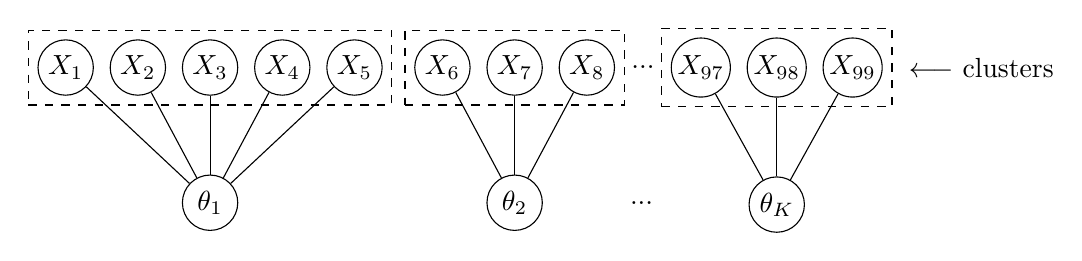
\begin{tikzpicture}[x=0.2cm]

  \FPeval{\spahalf}{clip(0.9)}
  \FPeval{\spamore}{clip(0.2)}

  \node[latent] (x-1)  {$X_1$} ;
  \foreach \i in {2,...,5}{
    \FPeval{\prev}{clip(\i - 1)}
    \node[latent, right=of x-\prev] (x-\i)  {$X_{\i}$} ;
  }
  \node[latent, right=of x-5, xshift=\spamore cm] (x-6)  {$X_6$} ;
  \foreach \i in {7,...,8}{
    \FPeval{\prev}{clip(\i - 1)}
    \node[latent, right=of x-\prev] (x-\i)  {$X_{\i}$} ;
  }
  \node[const, right=of x-8] (x-ellipsis)  {...} ;
  \node[latent, right=of x-ellipsis] (x-97)  {$X_{97}$} ;
  \node[latent, right=of x-97]       (x-98)  {$X_{98}$} ;
  \node[latent, right=of x-98]       (x-99)  {$X_{99}$} ;

  \gate {} {(x-1)(x-2)(x-3)(x-4)(x-5)} {}
  \gate {} {(x-6)(x-7)(x-8)} {}
  \gate {lastcluster} {(x-97)(x-98)(x-99)} {}
  \node[const, right=of lastcluster]    (cl-comment)  {$\longleftarrow$ clusters} ;

  \node[latent, below=of x-3]    (t-1)  {$\theta_{1}$} ;
  \foreach \i in {1,...,5}{
    \edge[-] {x-\i} {t-1}
  }
  \node[latent, below=of x-7]    (t-2)  {$\theta_{2}$} ;
  \foreach \i in {6,...,8}{
    \edge[-] {x-\i} {t-2}
  }
  \node[const, right=of t-2, xshift=\spahalf cm] (t-ellipsis)  {...} ;
  \node[latent, below=of x-98]    (t-k)  {$\theta_{K}$} ;
  \foreach \i in {97,...,99}{
    \edge[-] {x-\i} {t-k}
  }
  
\end{tikzpicture}

  \caption{Variable dependencies when learning one SVM per cluster (baseline used in Clustered SVM~\cite{gu2013clustered}).}
  \label{fig:gm-svmpercluster}
\end{figure}

\begin{figure}[h!]
  \centering
  \input{tikz-clusteredsvm}
  \caption{Variable dependencies for Clustered SVM~\cite{gu2013clustered}, where a common global regularization is used.}
  \label{fig:gm-clusteredsvm}
\end{figure}

\begin{figure}[h!]
  \centering
  
\newcommand{\mymul}[1]{{\mu}_{\mkern-0.66\thinmuskip\mathcal{L}, #1} }

\pgfdeclarelayer{bg}
\pgfsetlayers{bg,main}

\begin{tikzpicture}[x=0.2cm]

  \FPeval{\spahalf}{clip(0.9)}
  \FPeval{\spamore}{clip(0.2)}

  \node[latent] (x-1)  {$X_1$} ;
  \node[latent, below=of x-1] (mu-1)  {$\mymul{1}$} ;
  \foreach \i in {2,...,5}{
    \FPeval{\prev}{clip(\i - 1)}
    \node[latent, right=of x-\prev] (x-\i)  {$X_{\i}$} ;
    \node[latent, below=of x-\i] (mu-\i)  {$\mymul{\i}$} ;
  }
  \node[latent, right=of x-5, xshift=\spamore cm] (x-6)  {$X_6$} ;
  \node[latent, below=of x-6] (mu-6)  {$\mymul{6}$} ;
  \foreach \i in {7,...,8}{
    \FPeval{\prev}{clip(\i - 1)}
    \node[latent, right=of x-\prev] (x-\i)  {$X_{\i}$} ;
    \node[latent, below=of x-\i] (mu-\i)  {$\mymul{\i}$} ;
  }
  \node[const, right=of x-8] (x-ellipsis)  {...} ;
  \node[latent, right=of x-ellipsis] (x-97)  {$X_{97}$} ;
  \node[latent, right=of x-97]       (x-98)  {$X_{98}$} ;
  \node[latent, right=of x-98]       (x-99)  {$X_{99}$} ;
  \node[const, right=of mu-8] (mu-ellipsis)  {...} ;
  \node[latent, below=of x-97] (mu-97)  {$\mymul{97}$} ;
  \node[latent, below=of x-98] (mu-98)  {$\mymul{98}$} ;
  \node[latent, below=of x-99] (mu-99)  {$\mymul{99}$} ;
  \foreach \i in {1,...,8,97,98,99}{
    \edge[-] {x-\i} {mu-\i}
  }

  \gate {} {(x-1)(x-2)(x-3)(x-4)(x-5)} {}
  \gate {} {(x-6)(x-7)(x-8)} {}
  \gate {lastcluster} {(x-97)(x-98)(x-99)} {}
  \node[const, right=of lastcluster]    (cl-comment)  {$\longleftarrow$ clusters} ;

  
  % thetas
  \node[latent, below=of mu-3]    (t-1)  {$\theta_{1}$} ;
  \node[latent, below=of mu-7]    (t-2)  {$\theta_{2}$} ;
  \node[const, right=of t-2, xshift=\spahalf cm]   (t-ellipsis)  {...} ;
  \node[latent, below=of mu-98]    (t-k)  {$\theta_{K}$} ;
  \foreach \i in {1,...,5}{
    \edge[-] {mu-\i} {t-1}
  }
  \foreach \i in {6,...,8}{
    \edge[-] {mu-\i} {t-2}
  }
  \foreach \i in {97,...,99}{
    \edge[-] {mu-\i} {t-k}
  }

  % below
  \begin{pgfonlayer}{bg}
    \newcommand{\colorforb}{lightgray!75!blue}
    \newcommand{\colorforbb}{lightgray!75!green}
    \newcommand{\colorforL}{white!50!red}
    % b
    \node[latent, text=\colorforb, draw=\colorforb, below=of t-2, xshift=1.3cm]    (b)  {$\bm{b}$} ;
    \node[const, right=of b]    (b-comment)  {$\longleftarrow$ common bias} ;
    \foreach \i in {1,...,8,97,98,99}{
      \edge[-,color=\colorforb] {mu-\i} {b}
    }
    \edge[-,color=\colorforbb] {t-1} {b}
    \edge[-,color=\colorforbb] {t-2} {b}
    \edge[-,color=\colorforbb] {t-k} {b}
    % landmarks
    \node[latent, text=\colorforL, draw=\colorforL, right=of mu-99, xshift=0.5cm, yshift=-1.3cm] (L)  {$\bm{\mathcal{L}}$} ;
    %\edge[-,color=\colorforL] {mu-1} {L} % (no loop) good enough visually
    \foreach \i in {1,...,8,97,98,99}{
      \edge[-,color=\colorforL] {mu-\i} {L}
    }
    \node[const, right=of L]    (L-comment)  {$\longleftarrow$ landmarks} ;
  \end{pgfonlayer}

\end{tikzpicture}

  \caption{Variable dependencies for our model, \landSVM, where one SVM is learned per cluster but the local models interact through a common bias and $\mathcal{L}$, the set of landmarks.}
  \label{fig:gm-oursvm}
\end{figure}


\bibliographystyle{ieee}
\bibliography{paper}
\end{document}
